
\section{Requirements}

This chapter is used to explain the thoughts on the requirements that
 were made for the project. This covers analyzing what is involved in creating
  a game. The scope for the project will be covered and finally the use cases
   for the project will be introduced and explained.

\subsection{Game Development Analysis}

The following analysis covers games and gaming split into two parts.
The first part covers the concept of games. The second part covers the
issues with game development.\\\\
The concept of a game can be seen as a goal-oriented experience,
where a group of various activities is played out by one or more players.
These activities are to provide a form of enjoyment or pleasure through
 competition either with oneself or others. In order to keep the game
  consistent rules are imposed onto the game.
In this way, a game employs interactivity and participation of a user,
referred to as a player. The player is put into a scenario with rules and
 goals, where the scenario could be either a reference to or abstraction of
  a realistic situation. The player either gets a goal provided by the game,
   or the player creates their own goal. The goal must be completed to “win”
    the game. Getting into a position of inability or failure to complete the
     goal results in “losing” the game.\\\\
Developing a game can bring certain issues. One of those issues is
 presentation. If the player cannot effectively interact with or understand
  what they are seeing or reading, their experience may not lead to enjoyment.
   Another issue is interaction. Without the proper options to complete the
    required goals, the player may not be able to fulfill the goal. This can
     again lead to an undesirable experience. A third issue is efficiency. If
      the game is unplayable because of inefficiencies, or stability issues,
       the player may not even want to play the game.

\subsection{Scope}

The game will contain an online access functionality that utilizes
 a client-server structure connecting with a database, as the game will
  make use of user accounts for the client, it will be necessary to encrypt
   all user account information. The group choose to use .NET as the
    framework for developing the client-server structure, since C\# is used
     for programming. \\
The game will be very limited in graphics and aesthetics, since the
 focus of the development is on the technical aspects. The group have
  therefore chosen to limit the game to 2D graphics with very simple
   turn-based functionality, and make our own version of the classic
    board game Battleship. The group decided to make the game multiplayer
     to fulfill the distributed system part of the project.

\subsubsection{The Board Game}

The board game “Battleships” is build up around a basic turn based game,
with a grid size of 10x10. Before the game starts each player chooses the
 spot for each of their five ships. Each round a player chooses a coordinate
  to which he attacks from his side to the opponent side. If it is a hit, the
   opponent places a red pin in the boat that is a hit, and the same does the
    player who fired. If it is a miss, the firing player must place a white
     pin in the coordinate to show that the shot did not hit. Each player
      then have five ships in varying sizes up to five pins long. When a
       ship has been sunk the opponent must say what kind of ship that is
        down. When one of the players have lowered all the opponent's
         ships, they win.

\subsubsection{The Computer Game}

The computer game will incorporate the board game’s functionality,
 and make most of it automated. In the first round each player places
  their ships location on the boards’ grid. In the next rounds until a
   player has won, the players will switch turns when a tile has been
    chosen. During the current player’s turn, that player will be shown
     a larger version of the opponent’s grid with their ships locations
      hidden. The player will then choose a tile on the grid to reveal
       whether or not there is a ship. If there is a ship, the tile will
        be marked in red, if not the tile will be marked in gray. A player
         has won when all of the opponent's ships have been fully revealed.

\subsection{Use Case Diagram}

The use cases made for the project were assigned a category in order to
 differentiate between them. The categories were assigned after where the
  use cases’ functionality were most prevalent. UC means the code made for
   the client layer, US for server and lastly UD for database.

\subsubsection{Actors}

\textbf{Player}: Will be interacting with the system though the client.\\
\textbf{Client}: Software part that is responsible for the GUI and the connection
 to the Server. \\
\textbf{Server}: All the software logic will be located here\\
\textbf{Database}: Here the data will be stored.

\begin{figure}[h]
\centering
\includegraphics[scale=0.7]{usecase}
\caption{Usecase diagram}
\end{figure}
\clearpage

\subsection{Use Case Priority}

In order to prioritize our use cases, the group focused on three factors:
 First the amount we were going to learn from realizing the functionality
  involved. Second how important the use case is for fulfilling the
   requirement of the project. Lastly how important the functionality
    is for the final product, if some function is required in another
     use case as well. The more of these criteria, the use case fulfills,
      the higher it is prioritized.

\begin{figure}[h]
\centering
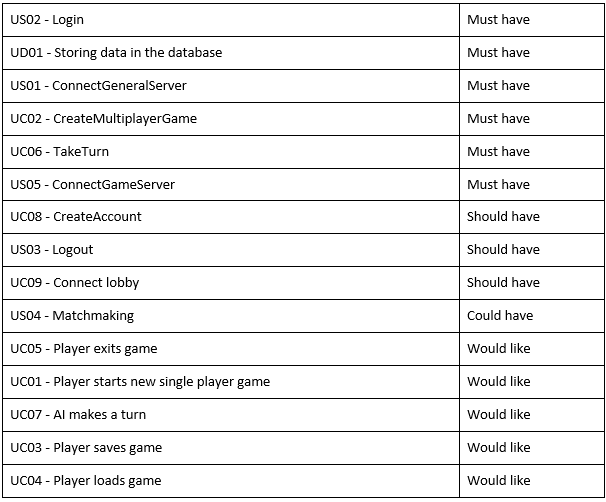
\includegraphics[scale=0.7]{Priority}
\caption{Usecase priority}
\end{figure}

\subsection{Use Case Description}

The report will be focusing on 2 use cases to show an idea of the thoughts
 behind the process.\clearpage

First one will be the creation of a game\\

\begin{figure}[h]
\centering
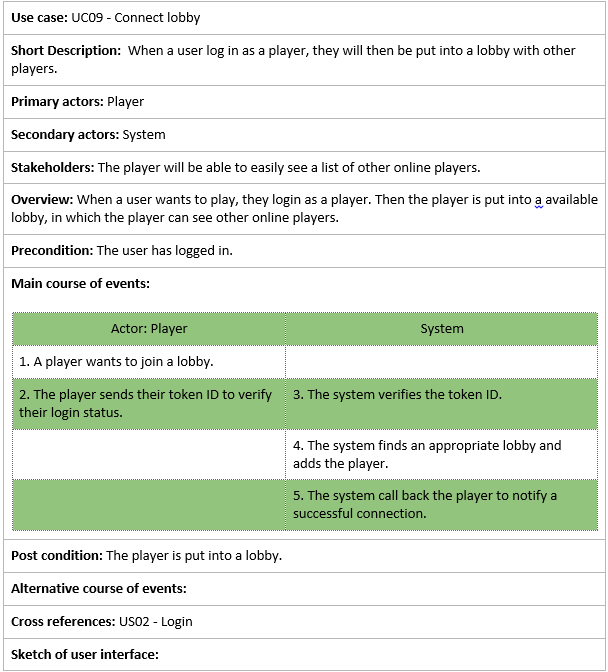
\includegraphics[scale=0.8]{usecon}
\caption{Usecase description for UC09}
\end{figure}
\clearpage

Second one is when the game is started and the player makes a turn.\\

\begin{figure}[h]
\centering
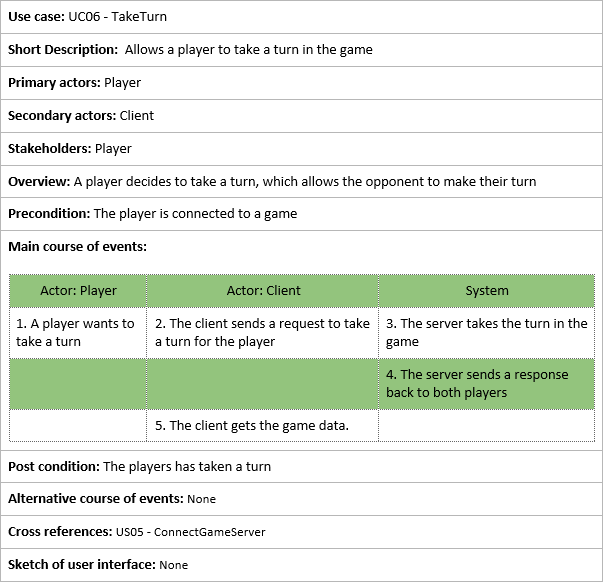
\includegraphics[scale=0.8]{usetak}
\caption{Usecase description for UC06}
\end{figure}
The remaning can be found in the appendix \ref{appendix:useCase_specification}
